\documentclass[a4paper, itemph]{oblivoir}
\setmainhangulfont{NANUMMYEONGJO.TTF}[BoldFont={NANUMMYEONGJOEXTRABOLD.TTF}]
\usepackage[english]{babel}
\usepackage[utf8x]{inputenc}
\usepackage[T1]{fontenc}
%% Sets page size and margins
\usepackage[a4paper,top=3cm,bottom=2cm,left=3cm,right=3cm,marginparwidth=2cm]{geometry}

\usepackage{indentfirst}

%% Useful packages
\usepackage{amsfonts}
\usepackage{amsmath, mathtools}
\usepackage{graphicx}
\usepackage{subcaption}
\usepackage[colorinlistoftodos]{todonotes}
\usepackage{amssymb}
\usepackage{amsthm}
\usepackage{tikz}

%Extravaganza
\newtheorem{thm}{Theorem}[subsection]
\newtheorem{lem}{Lemma}[subsection]
\newtheorem{cor}{Corollary}[subsection]
\newcommand{\overbar}[1]{\mkern 1.5mu\overline{\mkern-1.5mu#1\mkern-1.5mu}\mkern 1.5mu}
\theoremstyle{definition}
\newtheorem{defn}{Definition}[subsection]
\newtheorem{rem}{Remark}[subsection]

\begin{document}
\title{기초전자회로 및 실험: Lab \#07}
\author{서울대학교 전기$\cdot$정보공학부 2018-12602 이준협}
\maketitle

\section{Preliminaries}
This section serves as a short summary to the model of the drain current that this experiment uses, which was confirmed in lab 5. We note that since the drain is connected to $V_{DD}=8.12[V]$(batteries) and since the input voltage is less than $V_{DD}$, the transistor is always in saturation. 
\begin{equation}
     V_{sat}=\dfrac{V_{GS}-V_{TH}}{M}
\end{equation}
Equation (1) shows that $V_{DS}=V_{DD}-V_{out}>V_{in}-V_{out}=V_{GS}>\dfrac{V_{GS}-V_{TH}}{M}=V_{sat}$, since $M>1$. Now, the drain current at saturation is given by equation (2).
\begin{equation}
    I_{sat} = \dfrac{1}{2M}\dfrac{W}{L}C_{ox}\mu_n(V_{GS}-V_{TH})^2(1+\lambda V_{DS})
\end{equation}
Adjusting for body effect, the equations for $M$ and $V_{TH}$ in this model can be given as
\[M\approx 1+\dfrac{2.306}{\sqrt{0.6738+V_{SB}}+\sqrt{0.6738+V_{DB}}},\:V_{TH}=1.57+2.306(\sqrt{V_{SB}+0.6738}-\sqrt{0.6738})[V]\]
$\rho=2.306[V^{1/2}]$ and $2\phi_F=0.6738[V]$ were measured from the $V_{TH}-V_{SB}$ plot. We also use $\mu_n C_{ox}\dfrac{W}{L}=2500[\mu A/V^2]$, $\lambda = 1/35[V^{-1}]$ as a rough estimation from the values measured in lab 5.
\subsection{Large Signal Analysis}
To make the solution of the output voltage simpler, we linearize the equation for $V_{TH}$ as $V_{TH}=V_{TH,0}+\alpha V_{SB}=V_{TH,0}+\alpha V_{out}$. Then we have
\[
I_D=\frac{V_{out}}{R_S}=\dfrac{1}{2M}\dfrac{W}{L}C_{ox}\mu_n(V_{GS}-V_{TH})^2=\dfrac{1}{2M}\dfrac{W}{L}C_{ox}\mu_n(V_{in}-V_{TH,0}-(1+\alpha)V_{out})^2
\]
Solving this quadratic equation, we get
\begin{equation}
V_{out}=\dfrac{V_{in}-V_{TH,0}}{\alpha+1}+\dfrac{V_0}{2(\alpha+1)}-\dfrac{\sqrt{(\alpha+1)(V_{in}-V_{TH,0})V_0+\dfrac{V_0^2}{4}}}{(\alpha+1)^2}\text{ (}V_0=\dfrac{2ML}{R_S\mu_n C_{ox}W})
\end{equation}
We see that the output voltage is approximately linear, with a slope below unity, since $\alpha+1>1$.
\subsection{Small Signal Analysis}
Note that since $V_{DS}=V_{DB}-V_{SB}=V_{DD}-V_{SB}$, we have $dV_{DS}=-dV_{SB}$. Then the small signal model can be derived from calculating the total derivative of $I_D$ using $V_{GS}$ and $V_{SB}$ as independent variables.
\begin{align*}
    dI_D=&\dfrac{1}{M}\dfrac{W}{L}C_{ox}\mu_n(V_{GS}-V_{TH})(1+\lambda V_{DS})dV_{GS}\\
    &-\left\{\dfrac{1}{M}\dfrac{W}{L}C_{ox}\mu_n(V_{GS}-V_{TH})(1+\lambda V_{DS})\frac{\partial V_{TH}}{\partial V_{SB}}+\right.\\
    &\left.\dfrac{1}{2M}\dfrac{W}{L}C_{ox}\mu_n(V_{GS}-V_{TH})^2\lambda \right\} dV_{SB}
\end{align*}
We can write $g_m=\dfrac{1}{M}\dfrac{W}{L}C_{ox}\mu_n(V_{GS}-V_{TH})(1+\lambda V_{DS})$, $g_b=\dfrac{1}{M}\dfrac{W}{L}C_{ox}\mu_n(V_{GS}-V_{TH})(1+\lambda V_{DS})\dfrac{\partial V_{TH}}{\partial V_{SB}}=g_m\dfrac{\rho}{2\sqrt{V_{SB}+2\phi_F}}$, and $r_o=\dfrac{1/\lambda+V_{DS}}{I_D}$. Then the small signal gain can be given as
\begin{equation}
    A_v=\frac{\left(R_S||r_o||\dfrac{1}{g_b}\right)}{\dfrac{1}{g_m}+\left(R_S||r_o||\dfrac{1}{g_b}\right)}=\frac{1}{1+\dfrac{g_b}{g_m}+\dfrac{1}{g_m(r_o||R_S)}}=\frac{1}{1+\dfrac{\rho}{2\sqrt{V_{SB}+2\phi_F}}+\dfrac{1}{g_m(r_o||R_S)}}
\end{equation}
We calculate $g_m$, $r_o$ and $A_v$ as $g_m=\sqrt{\dfrac{2}{M}\dfrac{W}{L}C_{ox}\mu_n(1+\lambda V_{DS})I_{sat}}$, $r_o=\dfrac{1/\lambda+V_{DS}}{I_{sat}}$. Note that $V_{DS}=V_{DD}-V_{out}$, $I_{sat}=\dfrac{V_{out}}{R_S}$, so all we have to measure is $R_S$, $V_{in}$, and $V_{out}$ at the bias point.

\section{Voltage Transfer Curve}
\begin{figure}[htb]
    \centering
    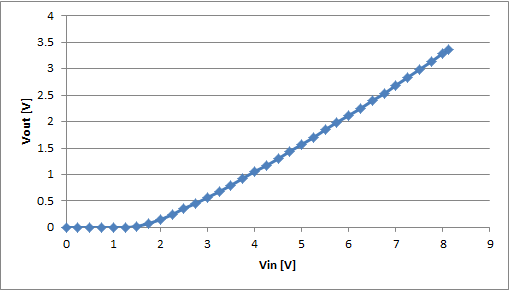
\includegraphics{vtc_cd.png}
    \caption{The voltage transfer curve of the CD amplifier}
\end{figure}
We use $R_S=10.01[k\Omega]$. We can see that the voltage stays at zero until the input voltage reaches the saturation voltage $V_{TH,0}$ at about $1.57[V]$, and then the voltage begins to rise at a rate below unity with a near-linear behavior. This fits in with equation (3), since $V_0=\dfrac{2M}{10.01\times 2.5}\approx \dfrac{4}{25}$ is small and $\alpha=\dfrac{\rho}{\sqrt{2\phi_F}+\sqrt{2\phi_F+V_{SB}}}>\dfrac{2.306}{\sqrt{3.5+0.6738}+\sqrt{0.6738}}\approx 0.8$ is moderately large, so the square root term, which changes sublinearly, affects the linear term only slightly.
\section{Small Signal Gain}

We observe that the output voltage of the amplifier is well-explained by the linear model, since $R^2=0.9997$ in figure 2. The input voltages are DC biases, since time-varying signals couldn't be given with a sufficiently constant frequency by hand. That is why changing the peak-to-peak voltage had no real significant meaning. The input voltage was given at $V_{in}=4.50\pm 0.50[V]$ and $V_{in}=4.50 \pm 1.00[V]$, and then all of the measurements were recorded on the graph in figure 2.
\begin{figure}[htb]
    \centering
    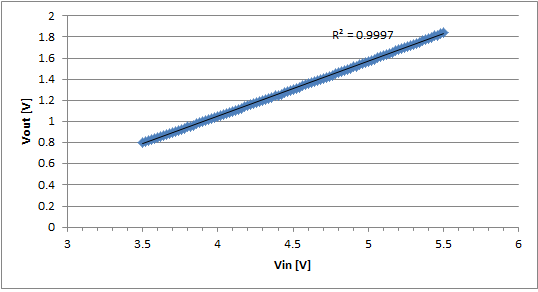
\includegraphics{10010_gain.png}
    \caption{Reaction of the CD amplifier with $R_S=10.01[k\Omega]$ when $V_{in}=4.50\pm 1.00[V]$, which is incremented by $0.02[V]$.}
\end{figure}

The measured gain when $\Delta V_{in}=1.00[V]$ was $\dfrac{1.567-1.048}{1.00}=0.52$, and the measured gain when $\Delta V_{in}=2.00[V]$ was $\dfrac{1.84-0.802}{2.00}=0.52$. Therefore, the gain did not change much according to the peak-to-peak voltage at the input. If the input was changing at a constant frequency, the gain might have changed due to the charging time of the input oxide capacitance, but since the output was measured at its DC steady-state value, such effects were not observable.
\begin{table}[htb]
    \centering
    \begin{tabular}{c|c|c|c|c|c|c|c}
         $R_S[k\Omega]$& $V_{in}[V]$ & $V_{out}[V]$ & $I_D[mA]$ & $g_m[mA/V]$ & $r_o[k\Omega]$ & $\dfrac{\rho}{2\sqrt{V_{SB}+2\phi_F}}$ & $A_v$ \\
         \hline
         10.01&4.50 & 1.303 & 0.1302 & 0.7165 & 321.3 & 0.8201 & 0.5092 
    \end{tabular}
    \caption{Theoretical small-signal gain calculated by $1/A_v=1+\dfrac{\rho}{2\sqrt{V_{SB}+2\phi_F}}+\dfrac{1}{g_mR_S}+\dfrac{1}{g_mr_o}$}
\end{table}

The small-signal gain, calculated with the method that adjusts $M$ and $V_{TH}$ according to $V_{SB}$, fits the measured value well. The approximate error is $\left|\dfrac{0.52-0.5092}{0.5092}\times 100\right|=1.92\%$. Thus, the body effect is enough to explain the small-signal gain well. The error is due to the non-linearity in the input-output transfer characteristic and due to the fact that $M$ also changes due to the changes in $V_{out}$.
\begin{thebibliography}{}

\bibitem{1} S. M. Sze and K. K. Ng, \textit{Physics of Semiconductor Devices}, 4th ed. Hoboken, NJ: Wiley, 2015.

\end{thebibliography}

\end{document}
